\chapter{Bases de Docker}
\label{ch:docker}

\section{Introduction}
Dans ce chapitre nous allons parler du fonctionnement de \emph{Docker} et \emph{Docker Compose}. Ce chapitre est réalisé sous le ton d'un cours d'introduction à Docker, afin de pouvoir transmettre les connaissances de base a l'utilisation et à la modification du travail réalisé lors de cette thèse. Cela passera entre autres par certains exemples et codes qui seront fournis en annexe notamment.

Docker permet l'exécution de code dans un conteneur indépendant de vote système hôte. 

\subsection{Utilisations}
\subsection{Compatibilité inter-OS}
Docker permet d'éviter les problèmes liés aux différences entre les environnements d'exécution. En effet, lorsque l'on exécute un code avec Docker ont contrôlé exactement l'état et le type d'environnement d'exécution. Cela rend donc possible l'exécution d'un code sous différent \gls{os} hôte (OSX, Linux, Windows).

Mais pourquoi ne pas utiliser une simple machine virtuelle ? Une première différence entre une machine virtuelle et Docker est le fait que Docker n'encapsule pas tout un \gls{os}, ceci permet une exécution beaucoup plus rapide, et c'est bien se que l'on cherche dans ce travail.

\begin{figure}[H] 
\centering 
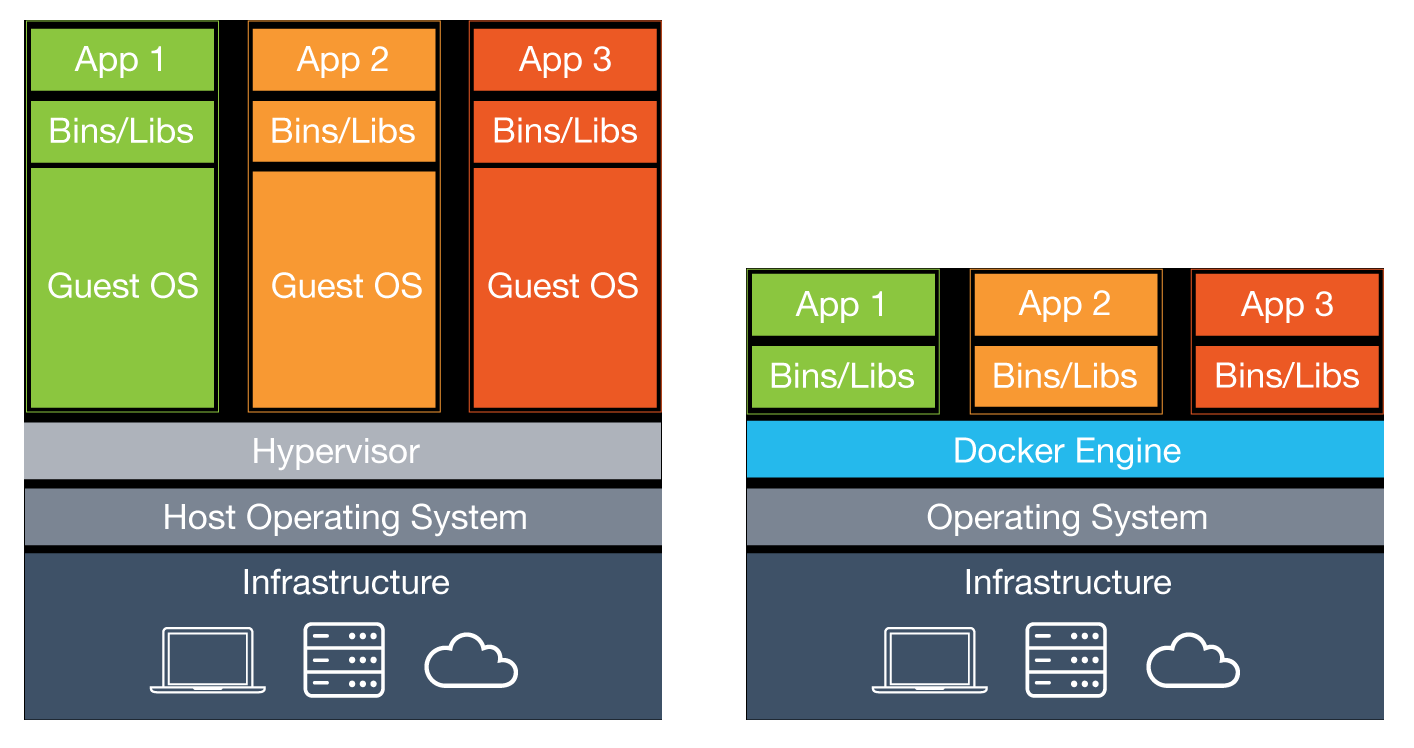
\includegraphics[width=1\columnwidth]{img/vm-vs-docker-container} 
\caption[vm vs Docker]{Virtual machine vs Docker}
\label{fig:vs} 
\end{figure}

\subsection{Miracle or illusion}
Je tiens ici à faire une mise en garde vis-à-vis de l'utilisation de Docker. Dans sont utilisation Docker est, à mon sens, une solution assez miraculeuse, notamment par le fait que l'on peu partage une application sans se poser de question sur l'hôte cible. Mais attention Docker n'est pas aussi miraculeux que cela dans le développement d'une solution applicative. En effet, il peut parfois êtres compliquer d'arriver du premier coup à réaliser se que l'on souhaite.

Docker n'est donc pas une solution miracle, mais présente beaucoup d'avantages en termes d'exécution standardisée, de partage de code et de déploiement.

\section{Pré-requis}
\subsection{Connaissance}
Il est nécessaire d'êtres à l’aise avec l'\gls{os} Linux et l'utilisation de commande UNIX. En effet, la plupart du temps les conteneurs utiliseront un système Linux. Pour plus d'information cf. ci-après.


\subsection{Installations}
\lstset{language=bash}
\lstset{
    frame=single,
    breaklines=true,
    postbreak=\raisebox{0ex}[0ex][0ex]{\ensuremath{\color{red}\hookrightarrow\space}}
}

\subsubsection{Installation Docker}
\begin{figure}[H] 
\centering 
\begin{lstlisting}[frame=single]
$ sudo apt-get update
$ sudo apt-get install apt-transport-https ca-certificates
$ sudo apt-key adv --keyserver hkp://p80.pool.sks-keyservers.net:80 --recv-keys 58118E89F3A912897C070ADBF76221572C52609D

$ sudo apt-add-repository 'deb https://apt.dockerproject.org/repo ubuntu-xenial main'
$ sudo apt-get update
$ sudo apt-cache policy docker-engine
$ sudo apt-get install -y docker-engine
$ sudo systemctl status docker
\end{lstlisting}
\caption[Code - Installation Docker]{Installation Docker}
\label{fig:installDocker} 
\end{figure}

Vous devriez maintenant voir une sortie console semblable a celle de la figure \ref{fig:dockerservices}:

\begin{figure}[H] 
\centering 
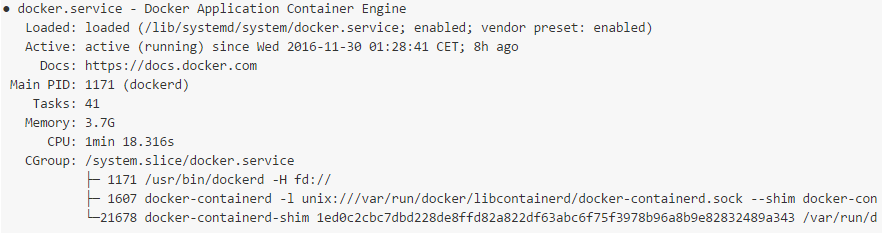
\includegraphics[width=1\columnwidth]{img/docker-services} 
\caption[docker services]{Services Docker opperationnel}
\label{fig:dockerservices} 
\end{figure}

Il faut à présent configurer Docker pour votre utilisateur hôte.

\begin{figure}[H] 
\centering
\begin{lstlisting}[frame=single]
$ sudo usermod -aG docker $(whoami)
\end{lstlisting}
\caption[Code - Configurer utlisateur Docker]{Configurer utlisateur Docker}
\label{fig:configUserDocker} 
\end{figure}

À se point ci, il vous faut redémarrer votre machine.

\subsubsection{Installation Docker-compose (1.9)}

\begin{figure}[H] 
\centering 
\begin{lstlisting}[frame=single]
$ curl -L "https://github.com/docker/compose/releases/download/1.9.0/docker-compose-$(uname -s)-$(uname -m)" -o /usr/local/bin/docker-compose
$ sudo chmod +x /usr/local/bin/docker-compose
$ docker-compose --version
\end{lstlisting}
\caption[Code - Installation Docker-compose]{Installation Docker-compose}
\label{fig:installCompose} 
\end{figure}

Vous devriez à présent obtenir la sortie console suivante:

\begin{figure}[H] 
\centering 
\begin{lstlisting}[frame=single]
docker-compose version: 1.9.0
\end{lstlisting}
\caption[Code - Docker-compose version]{Docker-compose version}
\label{fig:composeVersion} 
\end{figure}

\subsection{Téléchargements}

\section{Fonctionnement}
\subsection{Docker}
Il faut commencer par clarifier de quoi on parle lorsque l'on utilise le mot conteneur. Il s'agit d'une \emph{enveloppe} virtuelle permettant de packager une application ou un code avec toutes les dépendances nécessaires au fonctionnement de l'application. On package donc les fichiers source, librairies, runtime, outils, fichiers, base de données, etc. 

Un conteneur n'embarque pas de \gls{os}, il s'appuie sur celui de l'hôte sur lequel il est déployé. Ce qui rend un conteneur beaucoup moins lourd qu'une machine virtuelle \ref{fig:vs}.

Il faut également spécifier que Docker opère une isolation, des conteneurs, au niveau du système d'exploitation. 

Un conteneur Docker est décrit à l'aide d'un simple fichier \emph{.Dockerfile}, il décrit la création du conteneur, en détail. On peut personnaliser cette description de manière très détaillée. 

Il faut voir une application réalisée avec Docker comme une somme de microservices. Nous verrons dans la section suivante des exemples basiques d'application Docker. Le but étant de:

\begin{itemize}
\item rendre l'application davantage élastique;
\item améliorer les performances;
\item le déploiement continu est facilité. On peut relancer les services indépendamment les uns des autres.
\end{itemize}


\subsection{Docker-compose}
Docker-compose permet de définir et d'exécuter des applications multi-conteneurs. En effet, sans compose il fallait lancer les différents services de votre application soit manuellement soit en utilisant des scripts.

Compose utilise un fichier de composition, \emph{docker-compose.yml}, afin de configurer une application Docker. Ce qui permet de lancer une application à l'aide d'une seule commande. 

Pour résumer, une application Docker, utilisant Compose, est la combinaison de trois étapes:

\begin{enumerate}
\item Définir les différents Dockerfile des vos micro services composant l'application;
\item Définir les services qui seront utilisés dans le composé, leurs relations et leurs configurations;
\item Lancer l'application avec la simple commande, \emph{docker-compose up}.
\end{enumerate}

\section{Exemples}
\subsection{simple pull, build et run}
Les trois commandes les plus importantes de Docker sont \emph{pull}, \emph{build} et \emph{run}. En effet, ces commandes sont indispensables et doivent impérativement être comprises.

Premièrement, intéressons-nous à la commande \emph{pull}:

\begin{figure}[H] 
\centering 
\begin{lstlisting}[frame=single]
$ docker pull debian:jessie

jessie: Pulling from library/debian
5040bd298390: Pull complete 
Digest: sha256:abbe80c8c87b7e1f652fe5e99ff1799cdf9e0878c7009035afe1bccac129cad8
Status: Downloaded newer image for debian:jessie
\end{lstlisting}
\caption[Code - Docker pull]{Docker pull}
\label{fig:dockerPull} 
\end{figure}

Avec cette commande l'engin Docker à téléchargé l'image de debian Jessie depuis le \emph{Docker Hub}. Vous pouvez trouver un grand nombre d'images sur \emph{Docker Hub} - \hyperref[Docker Hub]{https://hub.docker.com/}.

Il est possible de gérer les images contenues sur une machine hôte. La commande suivante permet d'afficher la liste des images:

\begin{figure}[H] 
\centering 
\begin{lstlisting}[frame=single]
$ docker images

REPOSITORY           TAG                 IMAGE ID            CREATED             SIZE
debian               jessie              e5599115b6a6        2 weeks ago         123 MB
\end{lstlisting}
\caption[Code - Docker images]{Docker images}
\label{fig:dockerImage} 
\end{figure}

Il est également possible de supprimer une image, afin de libérer de l'espace disque:

\begin{figure}[H] 
\centering 
\begin{lstlisting}[frame=single]
$ docker rmi e5599115b6a6

Untagged: debian:jessie
Untagged: debian@sha256:abbe80c8c87b7e1f652fe5e99ff1799cdf9e0878c7009035afe1bccac129cad8
Deleted: sha256:e5599115b6a67e08278d176b05a3defb30e5564f5be6d73264ec560b484514a2
Deleted: sha256:a2ae92ffcd29f7ededa0320f4a4fd709a723beae9a4e681696874932db7aee2c
\end{lstlisting}
\caption[Code - Docker rmi]{Docker rmi}
\label{fig:dockerRmi} 
\end{figure}

Je tiens a signaler que l'on peut déjà se rendre compte d'un avantage de Docker par rapport a une machine virtuelle, l'image de Debian que l'on vient de télécharger ne fait que 123MB.

À présent lançons notre premier conteneur Docker:

\begin{lstlisting}[frame=single]
$ docker run -it debian:jessie /bin/bash

root@47e35436f723:/# 
\end{lstlisting}


Il est maintenant possible d'exécuter n’importe quelle commande à l'intérieur du conteneur:

\begin{lstlisting}[frame=single]
$ date

Sun Feb  5 11:01:11 UTC 2017
\end{lstlisting}

\emph{Ctrl+d} permet de sortir du conteneur.

\begin{figure}[H] 
\centering 
\begin{lstlisting}[frame=single]
$ docker run -itd debian:jessie

5c09ebfa8bc99235ad482256dfb9fa1fa470a42314ed61654b6a653aff6fee6b
\end{lstlisting}
\caption[Docker run linux]{Docker run linux}
\label{fig:DockerRunLinux} 
\end{figure}

En ajoutant l'option "d" le conteneur est exécuté de manière \emph{détachée}.

En utilisant la commande suivant, il est possible de visualiser les conteneurs en cours d'exécution:

\begin{figure}[H] 
\centering 
\begin{lstlisting}[frame=single]
$ docker ps

CONTAINER ID        IMAGE               COMMAND             CREATED              STATUS              PORTS               NAMES
5c09ebfa8bc9        debian:jessie       "/bin/bash"         About a minute ago   Up About a minute                       admiring_brattain
\end{lstlisting}
\caption[Docker ps]{Docker ps}
\label{fig:dockerPs} 
\end{figure}

Il est possible d'exécuter n’importe quelle commande dans un conteneur en cours d'exécution:

\begin{figure}[H] 
\centering 
\begin{lstlisting}[frame=single]
$ docker exec -it admiring_brattain date

Sun Feb  5 11:06:21 UTC 2017
\end{lstlisting}
\caption[Docker exec]{Docker exec}
\label{fig:dockerExec} 
\end{figure}

Ici le conteneur est identifié par son nom, si à l'exécution aucun nom n'est défini, Docker en attribue un de manière aléatoire. Il est également possible d'identifier un conteneur en utilisant son \emph{CONTAINER ID}.

En effet, il est possible et bien utile de définir un nom à vos conteneurs:

\begin{figure}[H] 
\centering 
\begin{lstlisting}[frame=single]
$ docker run -itd --name inphinity debian:jessie

c4be3f837adcbd5ab077e2b4a7903d2c1d4b5c434c7f877079c3ab5e22a2c555

$ docker ps

CONTAINER ID        IMAGE               COMMAND             CREATED             STATUS              PORTS               NAMES
c4be3f837adc        debian:jessie       "/bin/bash"         3 seconds ago       Up 3 seconds                            inphinity
\end{lstlisting}
\caption[Docker run]{Docker run}
\label{fig:dockerRun} 
\end{figure}

Finalement, abordons la commande \emph{build}. En effet, pour le moment nous n'avons fait qu'utiliser des images déjà construites. Un aspect très intéressant de Docker est de pouvoir décrire en détail la construction d'une image qui sera ensuite utilisée afin de lancer notre conteneur.

Prenons comme exemple le cas ou vous souhaité lancer un conteneur qui possède Python 3 préinstallé dans la version que l'on souhaite.

Pour se faire, il faut créer un fichier \emph{Dockerfile} dans un dossier vide. Vous pouvez retrouver le fichier de cet exemple dans le dossier "sources" et en annexe.

\begin{enumerate}
\item Il faut spécifier l'image de base:
\begin{lstlisting}[frame=single]
FROM debian:jessie
\end{lstlisting}

\item On souhaite premièrement mettre à jour les paquets:
\begin{lstlisting}[frame=single]
RUN apt-get update && \
    apt-get upgrade -y
\end{lstlisting}

\item Finalement, on installe le paquet que l'on souhaite, python dans sa version 3:
\begin{lstlisting}[frame=single]
RUN apt-get install -y python3
\end{lstlisting}

\end{enumerate}

À présent, on peut \emph{build} notre image Docker, l'exécuter et voir que python 3 est bien présent:

\begin{figure}[H] 
\centering 
\begin{lstlisting}[frame=single]
docker build -t exemple_1 .

[...]
Successfully built dead33da7d24

$ docker run -it exemple_1

root@41ac57ce9c0f:/# python3
Python 3.4.2 (default, Oct  8 2014, 10:45:20) 
[GCC 4.9.1] on linux
Type "help", "copyright", "credits" or "license" for more information.
>>> 

\end{lstlisting}
\caption[Docker build]{Docker build}
\label{fig:dockerBuild} 
\end{figure}

\subsection{Serveur Web: Docker compose}
Afin de montrer l'utilisation de \emph{Docker Compose} nous allons réaliser un petit serveur web. Cela nous permettra également de voir comment plusieurs microservices encapsulés chacun dans un conteneur Docker, peuvent former une application.

Toutes les sources de cet exemple sont disponibles dans le dossier, \emph{$sources/exemple_2$}.

Cet exemple consiste en deux conteneurs Docker, construit à partir de deux \emph{Dockerfile}.

Premièrement, un conteneur avec mysql, qui gère la base de données:

\begin{figure}[H] 
\centering 
\begin{lstlisting}[frame=single]
FROM mysql:5.7

COPY ./my.cnf /etc/mysql/conf.d/
\end{lstlisting}
\caption[mysql Docker]{Msyql Docker}
\label{fig:mysqlDocker} 
\end{figure}

Deuxièmement, un conteneur avec PHP et apache, afin d'exécuter les pages web:

\begin{figure}[H] 
\centering 
\begin{lstlisting}[frame=single]
FROM php:7-apache

COPY php.ini /usr/local/etc/php/

RUN apt-get update \
  && apt-get install -y libfreetype6-dev libjpeg62-turbo-dev libpng12-dev libmcrypt-dev \
  && docker-php-ext-install pdo_mysql mysqli mbstring gd iconv mcrypt
\end{lstlisting}
\caption[php-apache Docker]{php-apache Docker}
\label{fig:phpApacheDocker} 
\end{figure}

De plus, les sources se trouvent dans se que l'on appelle un volumes, une source de données pour nos conteneurs. Dans cet exemple nous y mettons uniquement un fichier \emph{index.php} avec la commande \emph{phpinfo()}, afin de vérifier que notre application fonctionne bien.

Nous allons utiliser \emph{Docker Compose}, afin de lancer notre application complète:

\begin{figure}[H] 
\centering 
\begin{lstlisting}[frame=single]
$ nano docker-compose.yml

version: '2'
services:
  mysql:
    build: ./mysql
    environment:
      MYSQL_ROOT_PASSWORD: pass
    volumes:
      - db:/var/lib/mysql
  php:
    build: ./php
    ports:
      - '8080:80'
    volumes:
      - ./html:/var/www/html
    depends_on:
      - mysql
volumes:
  db:

\end{lstlisting}
\caption[Code - docker-compose configuration]{docker-compose configuration}
\label{fig:composeConfig} 
\end{figure}

Exécutons, à présent, notre application web:

\begin{figure}[H] 
\centering 
\begin{lstlisting}[frame=single]
$ cd exemple_2/
$ docker-compose up -d

[...]

Creating exemple2_mysql_1
Creating exemple2_php_1

$ docker ps

CONTAINER ID        IMAGE               COMMAND                  CREATED             STATUS              PORTS                  NAMES
e921dc5930ac        exemple2_php        "docker-php-entrypoin"   4 minutes ago       Up 4 minutes        0.0.0.0:8080->80/tcp   exemple2_php_1
cdb19eaa3cb7        exemple2_mysql      "docker-entrypoint.sh"   4 minutes ago       Up 4 minutes        3306/tcp               exemple2_mysql_1

\end{lstlisting}
\caption[Docker-compose up]{Docker-compose up}
\label{fig:composeUp} 
\end{figure}

Pour vérifier que tous fonctionnent, utilisez votre navigateur favori et accédez à l'adresse \emph{localhost:8080} \ref{fig:phpinfo}.

\begin{figure}[H] 
\centering 
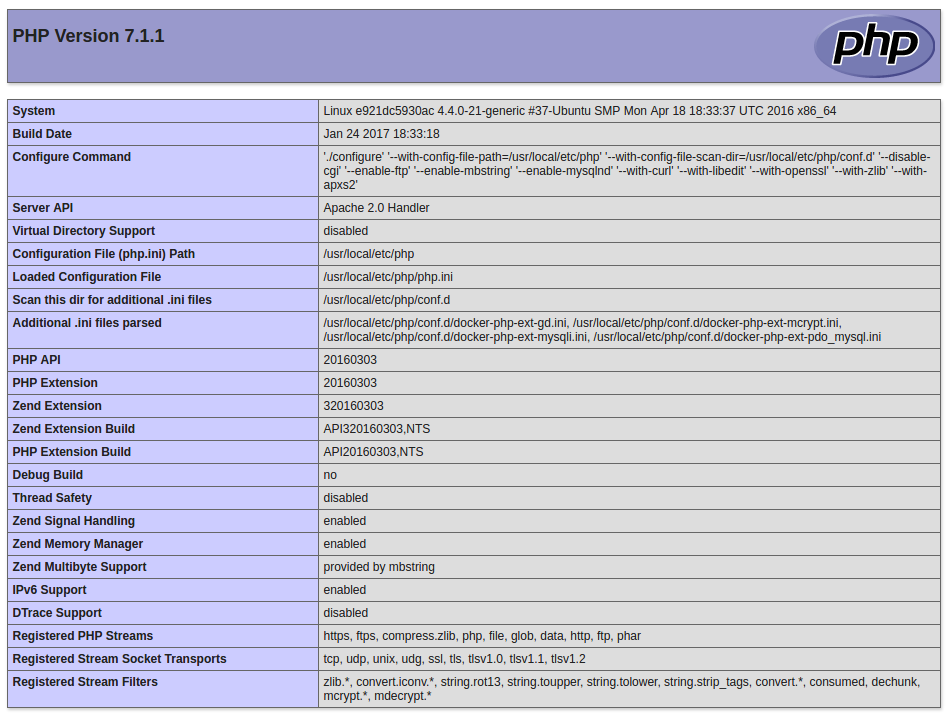
\includegraphics[width=1\columnwidth]{img/phpinfo} 
\caption[phpinfo]{phpinfo()}
\label{fig:phpinfo} 
\end{figure}

\subsection{Parallélisation}

Il est possible de lancer plusieurs conteneurs avec la même image. Nous allons utiliser ceci dans la suite du développement afin de lancer plusieurs conteneurs pour l'analyse des séquences.

\begin{figure}[H] 
\centering 
\begin{lstlisting}[frame=single]
$ docker run -itd debian:jessie

kamyh@kamyh-linux-tower ~/projects/master/documents/sources/exemple_2 $ docker ps
CONTAINER ID        IMAGE               COMMAND             CREATED             STATUS              PORTS               NAMES
8901929d2bf0        debian:jessie       "/bin/bash"         2 seconds ago       Up 1 seconds                            determined_sinoussi
877d2cddce6d        debian:jessie       "/bin/bash"         3 seconds ago       Up 2 seconds                            boring_nobel
4ff340b9c797        debian:jessie       "/bin/bash"         4 seconds ago       Up 3 seconds                            loving_mccarthy
e9a8bda7688f        debian:jessie       "/bin/bash"         4 seconds ago       Up 3 seconds                            focused_dijkstra
2060301458d6        debian:jessie       "/bin/bash"         5 seconds ago       Up 5 seconds                            awesome_blackwell
\end{lstlisting}
\caption[Docker Hmmer]{Docker Hmmer}
\label{fig:dockerHmmer} 
\end{figure}

Ici nous avons cinq conteneurs debian lancé simultanément. Ceci peut être très utile, par exemple, dans le cas d'une application web, afin de partager la charge des connexions utilisateurs entre plusieurs conteneurs.
































